\section{Experiments and results}

In this section we examine the results of the baccalaureates held in 2019, 2020 and 2021. Since the difficulty level of the individual exam modules varies each year, we believe that through combining the results from the three years we obtain data that is more representative of the general baccalaureate exam.

\begin{table}[!b]
  \caption{Number of participants at the Romanian Baccalaureate}
  \label{group-size}
  \centering
  \begin{tabular}{l|llll}
    \toprule
    Student group & Size (2019) & Size (2020) & Size (2021) & Total size \\
    \midrule
    \textit{R} & 121 693 & 140 315 & 120 472 & 382 480 \\
    \textit{M} & 6 826 & 7 351 & 6 381  & 21 528 \\
    \bottomrule
  \end{tabular}
\end{table}

\begin{table}[!b]
  \caption{Average final grades at the Romanian Baccalaureate}
  \label{group-average}
  \centering
  \begin{tabular}{l|llll}
    \toprule
    Student group & Average (2019) & Average (2020) & Average (2021) & Total average \\
    \midrule
    \textit{R} & 7.007 & 6.820 & 7.030 & 6.946 \\
    \textit{M} & 6.868 & 6.994 & 7.013 & 6.958 \\
    \bottomrule
  \end{tabular}
\end{table}

We denote the group of students who had to take only three written exams as \textit{R}. Those studying one of the minority languages are treated as a single group \textit{M} because they share the common trait of having four exams instead of three. It must be noted that their actual distribution is similar to the one presented in subsection \ref{ssec:min}, with Hungarians accumulating to 5.3\% of exam participants and all of the other minorities totalling up to 0.7\%. 

Table \ref{group-size} shows the number of the students not disqualified from any of the exams (i.e. with valid grades). Table \ref{group-average} displays the average final grades of the two groups in each year. Although we can not tell whether or not the grades of \textit{M} would be greater if they only had to take three exams, we observe that the difference between the average final grades of \textit{R} and \textit{M} is very small. Therefore, based on these three years' data, \textit{M} does not seem to be at disadvantage when considering only the final grades.
 
 
\begin{figure}[!b]
    \centering
    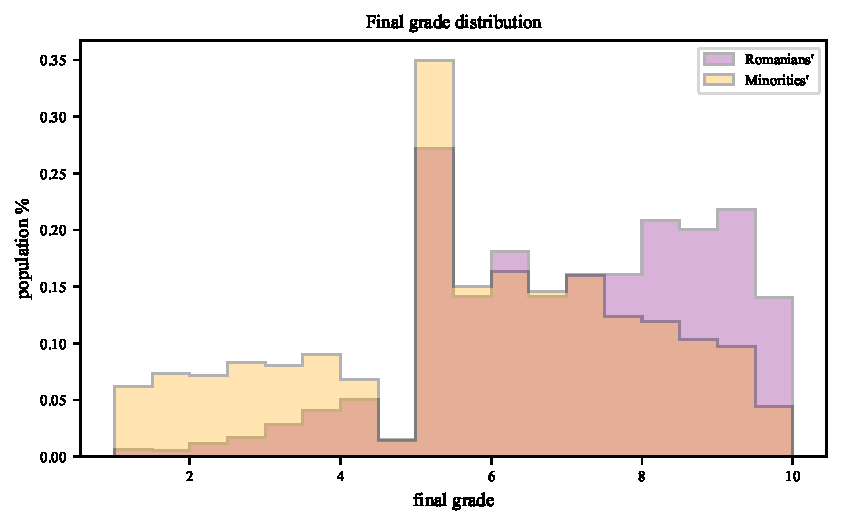
\includegraphics[width=14cm]{plots/exp4_grade_distrib.pdf}
    \caption{Distribution of the Romanian language and literature grades}
    \label{fig:ro-distr}
\end{figure}

\begin{figure}[!b]
    \centering
    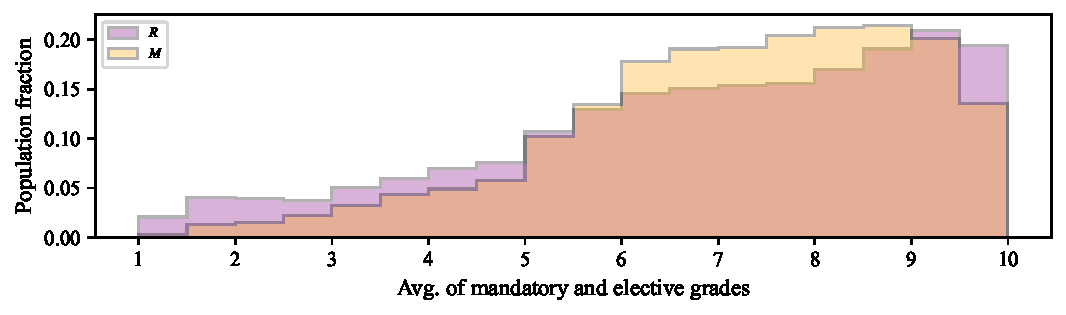
\includegraphics[width=14cm]{plots/exp4_grade_distrib_spec.pdf}
    \caption{Distribution of the average of the mandatory and elective subject grades}
    \label{fig:subj-distr}
\end{figure}


The distribution of the final grades in Romanian language and literature is shown in Figure \ref{fig:ro-distr}. A notable aspect of this distribution is that there are relatively few grades between 4 and 5 and many grades between 5 and 5.5. A probable explanation for this is that teachers correcting the exam might be less strict when the student's grade would otherwise fall right below the minimum passing grade.

The plot shows that group \textit{M} achieves worse grades than \textit{R} on this particular exam. The average grade in this subject for \textit{R} is 7.060, while for \textit{M} it is 5.744. Thus, on average, group \textit{R} achieves a grade greater by 1.316, which equates to a difference of 14.62\%.

% If the Romanian literature grades contain such a big discrepancy between \textit{M} and \textit{R}, yet the average final grades are close, something must account for this difference. \textit{M}'s average grade in their mother tongue language and literature exam is 7.630.

It is worth comparing \textit{M}'s grade in their native language and literature to \textit{R}'s Romanian literature grade. \textit{M}'s average native language grade is 7.630, which is greater by 0.570 than the average Romanian grade of \textit{R} and by 1.886 than the average Romanian grade of \textit{M}. Yet, this greater native literature grade does not fully account for how group \textit{M} makes up for their lesser Romanian literature grades to have an almost even average final grade. 

Figure \ref{fig:subj-distr} shows that the rest of the discrepancy between the two groups lies in their specialisation-specific grades. Proportionally to their sizes, \textit{M} achieves considerably more grades in the 6 to 9 grade buckets, summing up to a 0.294 higher average grade in the two specialization-specific exams. Specifically, \textit{R}'s average is 6.888 as opposed to \textit{M}'s 7.182.

This difference is not negligible, since the mandatory and elective exams of the specialisation should have very little to do with the participants' native languages. The phenomenon could have several different explanations: minority schools might better prepare students for their study profile exams, or the minority exam graders could be less strict.


\begin{figure}
    \centering
    \begin{minipage}[t]{0.49\textwidth}
        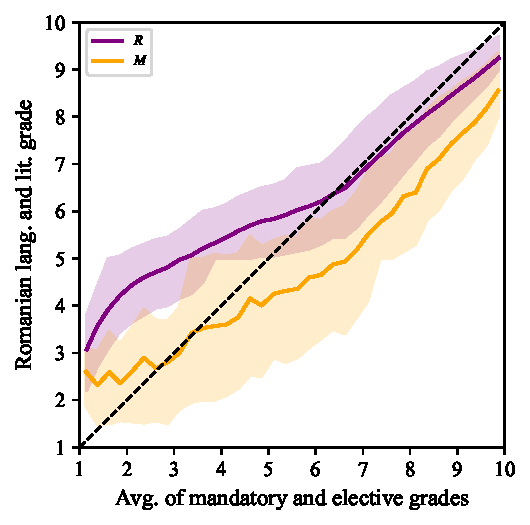
\includegraphics[width=7cm]{plots/exp1_grade_plot.pdf}
        \caption{Expected Romanian language and literature grades given the average of the specialisation's mandatory and elective grades}
        \label{fig:ro-vs-subj}
    \end{minipage}
    \hfill
    \begin{minipage}[t]{0.49\textwidth}
        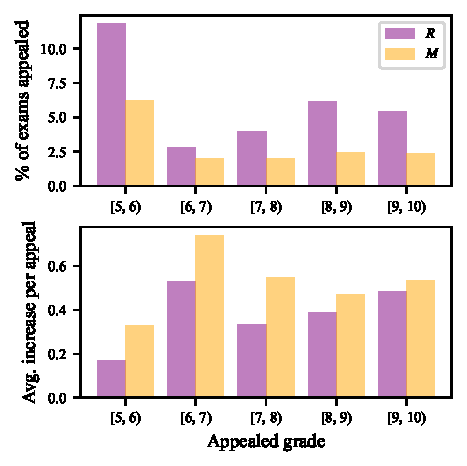
\includegraphics[width=7cm]{plots/exp6_appeal_ro.pdf}
        \caption{Percentage of students in each grade group submitting a grade appeal for their Romanian lang. and lit. exam (top). Average increase in grade after the appeal (bottom)}
        \label{fig:appeal}
    \end{minipage}
\end{figure}



Figure \ref{fig:ro-vs-subj} is achieved by separating the examinees into 36 groups based on the average of the grades specific to their study profiles and computing the average Romanian language grade for each group. Additionally, the plot also shows the area bounded by the 25\textsuperscript{th} and 75\textsuperscript{th} percentiles.

We can observe that in the case of both \textit{M} and \textit{R} better specialisation grades generally lead to better grades on the Romanian exam. Supporting the assumption that better \textit{M} students are at a lesser disadvantage at the Romanian literature exam, we can notice that the difference does tighten between the Romanian grades of \textit{M} and \textit{R} when their average specialisation grade is above 8.

% Yet, the minority native grade is higher than the average Ro grade. Again, can use Cohen's d effect size.

% Language skills

% Specialisations

Our last assumption underlined in subsection \ref{ssec:motiv} is regarding the improper treatment of Romanian language and literature grade appeals submitted by \textit{M} members. What the top part of Figure \ref{fig:appeal} reveals is that only a considerably smaller percentage of \textit{M} requests a grade appeal in this exam module. Presumably, they require more confidence in a successful re-evaluation. This is a feasible explanation to the bottom plot of the figure, namely that \textit{M} receives on average a higher increase in their final grade from their grade appeals.




